\chapter{Grundlagen}
\label{background}

Im folgenden Kapitel werden einige Grundlagen dargelegt, welche für das weitere Verständnis der Arbeit relevant sind. Nach einer Einführung in die Funktionsweise und Rollenverteilung bei Pen-\&-Paper-Rollenspielen und deren Abgrenzung zu ihren digitalen Gegenstücken werden ähnliche Arbeiten vorgestellt und abgegrenzt. Insbesondere werden Limitationen vorhandener Implementierungen aufgezeigt und Ansätze zur Aufhebung dieser Grenzen vorgestellt.
%Alle Quellen hier referenzieren!

%- Allgemeine Wissensgrundlagen des Fachgebiets
%- Spezielle Grundlagen, die für das Verständnis erforderlich sind
%- Rahmenbedingungen für die Arbeit
%- Ausführungen zum Stand des Wissens / der Technik
%Als Leitprinzip gilt: Nur Informationen erwähnen, die
%- später benötigt werden,
%- notwendig sind, um die Arbeit oder ihre Motivation zu verstehen
%Das heißt insbesondere,
%- keine Inhalte aus Lehrbüchern, außer
%- diese werden benötigt, um Problemstellung oder Lösungsweg zu definieren.

%Was sind Pen&Paper spiele?
%Was tun die Spieler?
%Was tut der Spielleiter?


\section{Pen-\&-Paper-Spiele}
\label{sec:PenPaperSpiele}

%\begin{itemize}
%	\item Kurze Erklärung wie so etwas abläuft
%	\item Übersicht über bekannte PnP Spiele, was ist an D\&D besonders?
%	\item \textit{[Abgrenzung zu normalen RPGs]} NEIN, da in \ref{sec:DigitaleRollenspiele}
%\end{itemize}

\begin{figure}[hbtp]
	\centering
		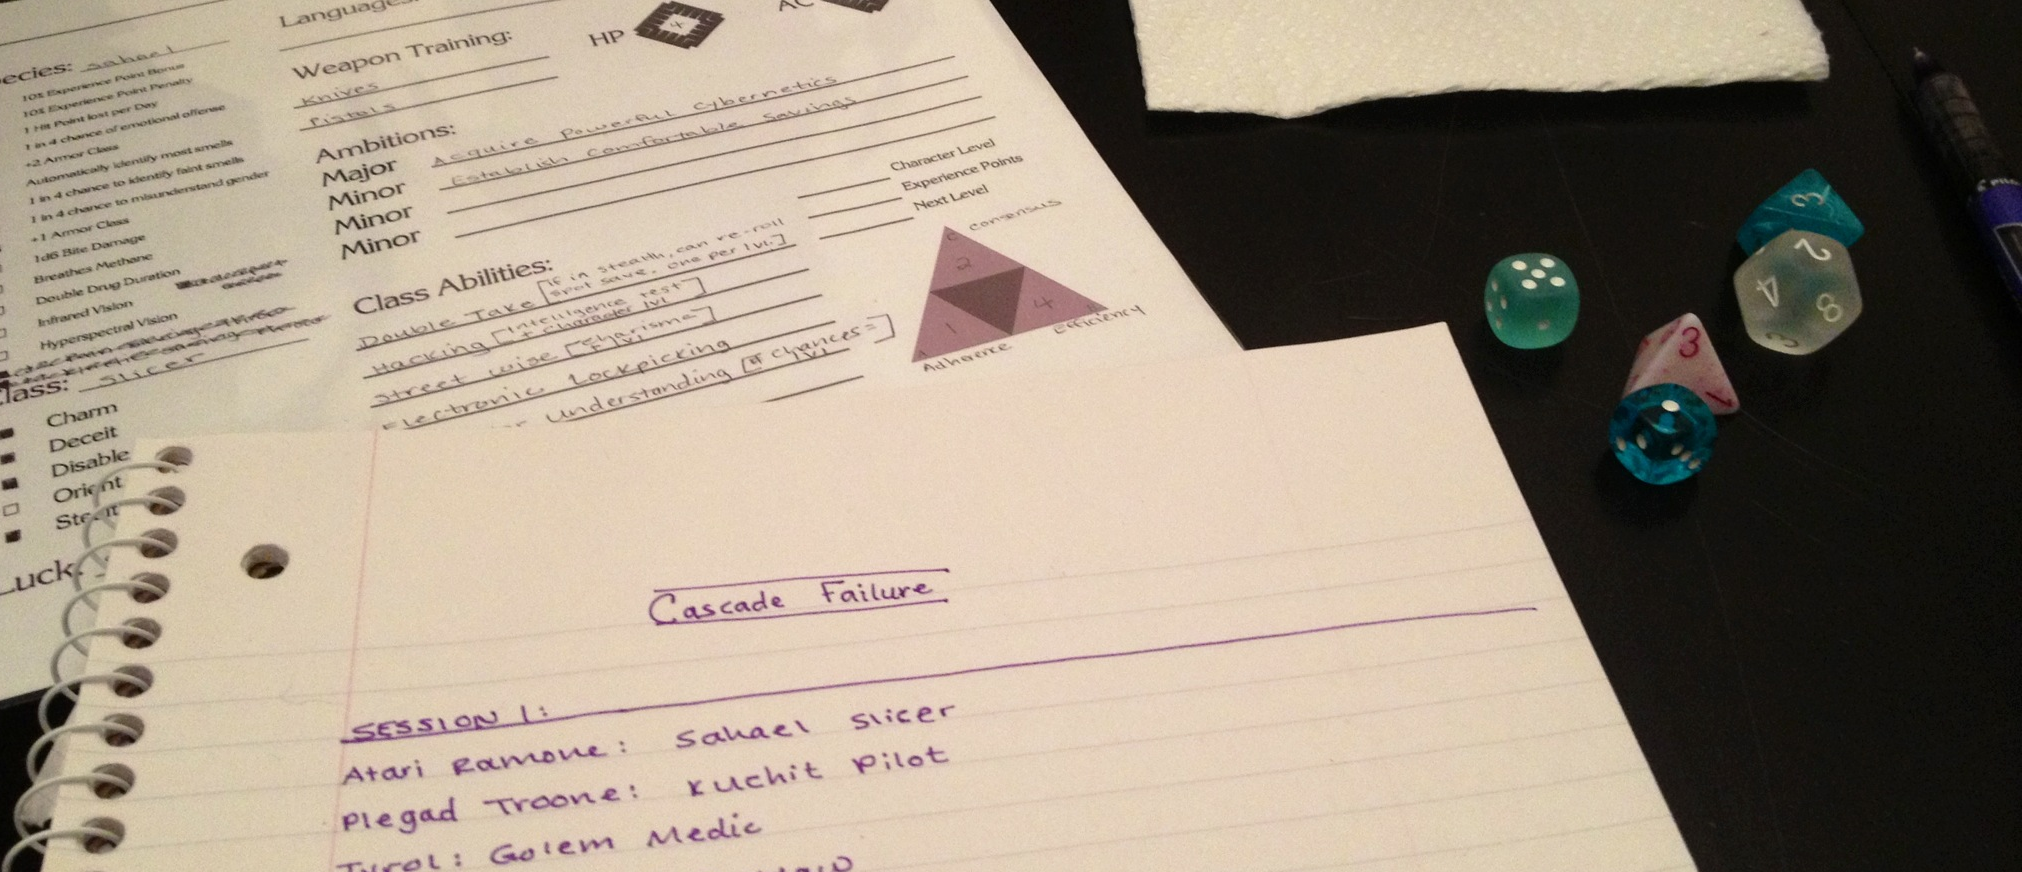
\includegraphics[width=1.00\textwidth]{media/pnp_supplies.png}
	\caption [Typische Ausrüstung bei einer Pen-\&-Paper-Spielrunde: Würfel, Notizen und Charakterbogen.]{Typische Ausrüstung bei einer PnP-Spielrunde: Würfel, Notizen und Charakterbogen.\protect\footnotemark[1]}
	\label{fig:pnp_supplies}
\end{figure}

\footnotetext[1]{http://eclectickellycole.wordpress.com, 20.03.14}
\addtocounter{footnote}{1}

Pen-\&-Paper-Rollenspiele (im folgenden auch als PnP bezeichnet) stellen eine Urform des Rollenspiels dar \cite{Apperley2006}. Mehrere Spieler treffen sich um gemeinsam ein Abenteuer zu erspielen. Einer der Spieler nimmt dabei die Rolle des Spielleiters ein. Die Spieler werden von dem Spielleiter durch ein fiktives Abenteuer geführt, wobei in der Regel der genaue Verlauf der Geschichte stark von der Interaktion der Mitspieler abhängt. \cite{Apperley2006}\newline 
Eine Besonderheit von PnP-Rollenspielen ist, dass keinerlei reales Rollenspiel stattfindet. Zwar erhalten die Spieler oftmals begleitende Materialien wie etwa Karten vom Spielleiter, das eigentliche Spiel findet jedoch in der Phantasie der Spieler statt \cite{Copier2005}. Die Interaktion mit der Spielwelt erfolgt verbal, Spieler treffen Aussagen über Aktionen die der Charakter ausführen soll. Der Spielleiter validiert diese Aussagen und antwortet mit dem Resultat der Aktion. Durch diese Art der Kommunikation ergibt sich oftmals ein dynamischen Abenteuer, welches speziell auf die Spielergruppe zugeschnitten ist. \cite{Drachen2008}\newline
Eines der ältesten und wohl auch bekanntesten PnP-Regelsysteme ist das 1974 vorgestellte \emph{Dungeons \& Dragons} (kurz \emph{D\&D}). Dieses Regelsystem vereint die damals sehr populären \emph{Wargames} mit dem literarischen Fantasy-Genre \cite{Copier2005}. Die Kernregeln von D\&D in der Version 3.5 wurden vom Verlag \emph{Wizards of the Coast} unter der liberale d20-Lizenz frei veröffentlicht~\cite{SRD35}.


\subsection{Spielleiter}
\label{sec:Spielleiter}
%Beschreibung der Tätigkeiten und Funktion von Spielleitern beim PnP\newline
%Abdecken von:
%\begin{itemize}
%	\item Konzeption und Umsetzung eines Abenteuers ('offline' vor der Spielrunde)
%	\item Durchführen des Spieles ('online' währen der Runde mit dem Spielern zusammen)
%\end{itemize}
Der Spielleiter hat bei einem PnP-Rollenspiel die Aufgabe eine Geschichte für die Spielrunde zu erdenken und die Teilnehmer während des Verlaufes anzuleiten. Im Vorfeld der Spielrunde konzipiert der Spielleiter dafür in der Regel eine Ausarbeitung eines Abenteuers. Meist werden hierfür Kerncharaktere und wichtige Entscheidungspunkte und Szenen ausgearbeitet, während sich der genaue Verlauf des Abenteuers beim Spielen ergibt. \ref{fig:storyflow_pnp} zeigt, wie sich aus mehreren Ideen des Spielleiters durch Einflussnahme und Interaktion der Spieler eine Geschichte ergibt. Die Darstellung veranschaulicht, wie der Spielleiter verschiedene Eckpunkte ausgearbeitet hat~(D1-En) welche durch die Interaktionen der Spieler und Geschehnisse wahrgenommen oder verworfen werden und somit die erlebte Geschichte ergeben~(A, B und C). Um diese Entwicklung zu ermöglichen muss der Spielleiter verschiedene Funktionen erfüllen.\newline
\cite{Arinbjarnar} nennt drei verschiedene Kernaufgaben des Spielleiters: \emph{Storyteller}, \emph{Actor} und \emph{Judge}. Zum einen ist es die Aufgabe des Spielleiters die Geschichte aus objektiver Sicht zu erzählen und die Handlung mit den Spielern voranzutreiben. Gleichzeitig nimmt er jedoch auch die Rolle und den Standpunkt aller NSCs ein und vermittelt zwischen ihnen und den Spielern. Als letzte Aufgabe achtet der Spielleiter auf die Einhaltung aller Regeln und trifft Entscheidungen falls es zu Unstimmigkeiten kommt.
\begin{figure}
	\centering
		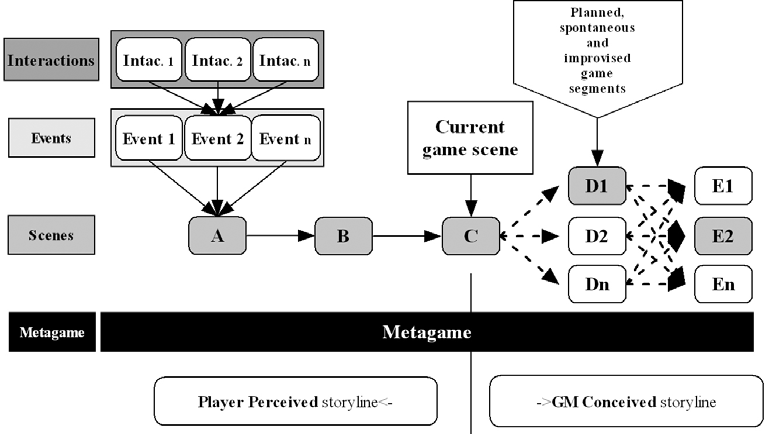
\includegraphics[width=1.00\textwidth]{media/storyflow_pnp.png}
	\caption{Entwicklung eines Pen-\&-Paper-Abenteuers im Verlauf der Spielrunde nach \cite{Tychsen2006a}.}
	\label{fig:storyflow_pnp}
\end{figure}


\subsection{Spielermotivation}
\label{sec:Spielermotivation}

%\begin{itemize}
%	\item Hervorheben was die PnP Spieler wollen (nach Möglichkeit belegen: Paper, Foren, unsere Testspieler, Pathfinder Entwickler)
	%	\begin{itemize}
%		\item Kreative Interaktive Geschichte
%		\item Soziale Komponente
%		\item 'Gemeinsam Abenteuer erleben'
%	\end{itemize}
%\end{itemize}
Im Gegensatz zu digitalen Rollenspielen geht es den Spielern von PnP-Rollenspielen meist weniger um die Charakterprogression oder das Absolvieren von \emph{Quests}, sondern um das gemeinsame Erleben einer interaktiven Geschichte. Die Geschichte kann durch Entscheidungen von Spielern aktiv mitgestaltet werden indem sie durch Rollenspiel die von dem Spielleiter vorgestellten Szenarien ausfüllen. Eine Spielergruppe kann so den Pfad eines Abenteuers relativ frei ausgestalten. Zwar ist die Geschichte in Grundzügen geplant, aber die Spieler entscheiden sich immer wieder aufs Neue welchen Weg sie wählen möchten. \cite{Arinbjarnar}\\
Die Freiheit eigene, nicht standardisierte Handlungen umsetzen zu lassen und in der Gruppe auf die teils unvorhersehbaren Konsequenzen zu reagieren stellt den Reiz von PnP-Spielen dar. 


\subsection{Gängige Spielmechaniken}
\label{sec:Spielmechaniken}

In den meisten PnP-Regelwerken ist es üblich viele Aktionen mit einem Zufallsfaktor zu versehen. Dazu werden Würfel unterschiedlicher Größenordnung und Anzahl verwendet. Ein Würfel mit 6 Seiten wird durch \textit{W6} abgekürzt, weitere Würfel sind zum Beispiel \textit{W2} (eine Münze), \textit{W4}, \textit{W8}, \textit{W10}, \textit{W12} und \textit{W20}.\newline
Charaktere besitzen überdies Fähigkeiten deren Werte mit denen eines Würfelwurfes verrechnet werden und den Ausgang einer Aktion beeinflussen. Das Ergebnis einer Rechnung wird dann mit einem durch andere Charaktere berechneten oder vom Regelwerk oder Spielleiter festgelegten Wert verglichen. Dieses Vorgehen wird als Probe bezeichnet und kann einen erfolgreichen, wirkungslosen oder fatalen Ausgang nehmen.\newline
Für besonders gelungene Spielzüge kann der Spielleiter Erfahrung verteilen. Je nach Spielweise werden zusätzlich Ressourcen und Lehrer benötigt um mit diesen Punkten Fähigkeiten zu steigern und damit den Charakter zu entwickeln. Dadurch können Proben besser absolviert oder erst ermöglicht werden.

Eine Besonderheit von PnP-Spielen im Vergleich zu digitalen Rollenspielen ist, dass sie auf keine allgemeingültige Repräsentation der Spielwelt zurückgreifen können. Das eigentliche Spiel findet nur in der Fantasie der Spieler statt. Daher ist die Kommunikation zwischen den Spielern ein wichtiges Instrument um das eigenen Verständnis der Spielwelt abzugleichen und um geplante Aktionen an den Spielleiter weiterzugeben. \cite{Drachen2008}

\section{Digitale Rollenspiele}
\label{sec:DigitaleRollenspiele}
%
%Beschreibung eines Standard Pc-Rollenspiels mit Mechaniken und Möglichkeiten\newline
%Dient später der Abgrenzung zu unserem Prototyp
%\begin{itemize}
%	\item DSA Reihe
%	\item D\&D Online
%	\item Neverwinter Nights
%	\item Elder Scrolls
%	\item Baldurs Gate
%	\item Icewind Dale
%\end{itemize}
%Besonders auf die D\&D basierten eingehen, den rest nur als Beispiele für andere Systeme.

\begin{figure}[h]
	\centering
	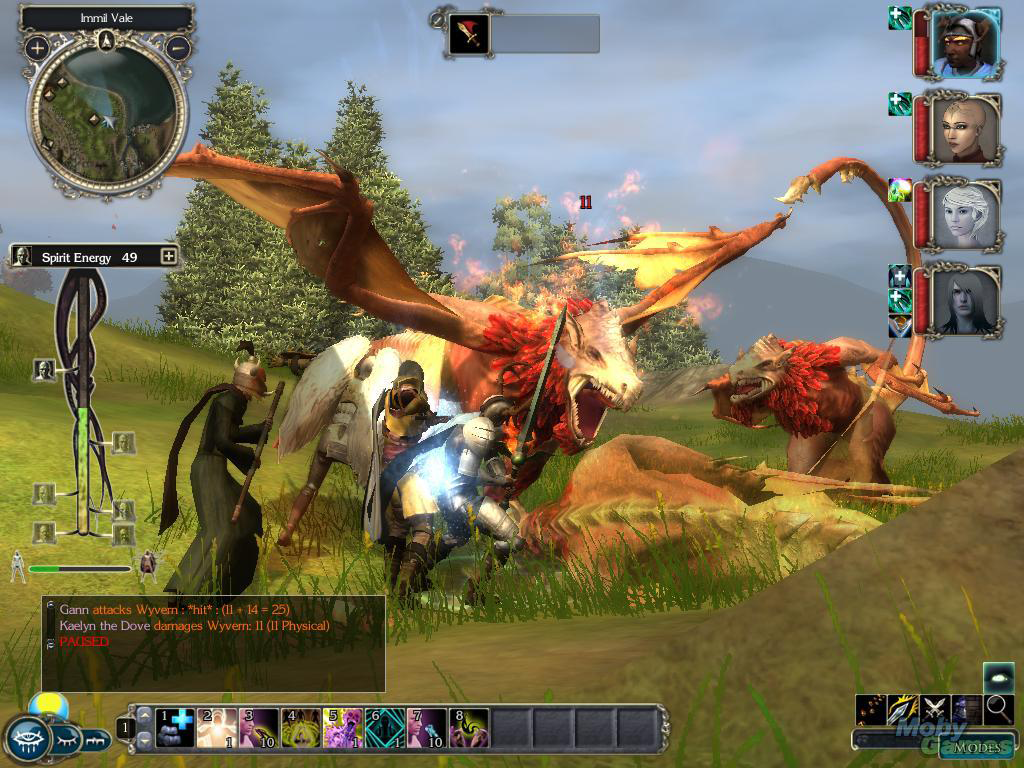
\includegraphics[width=0.465\textwidth]{media/NeverwinterNights2-game}\hspace{0.008\textwidth}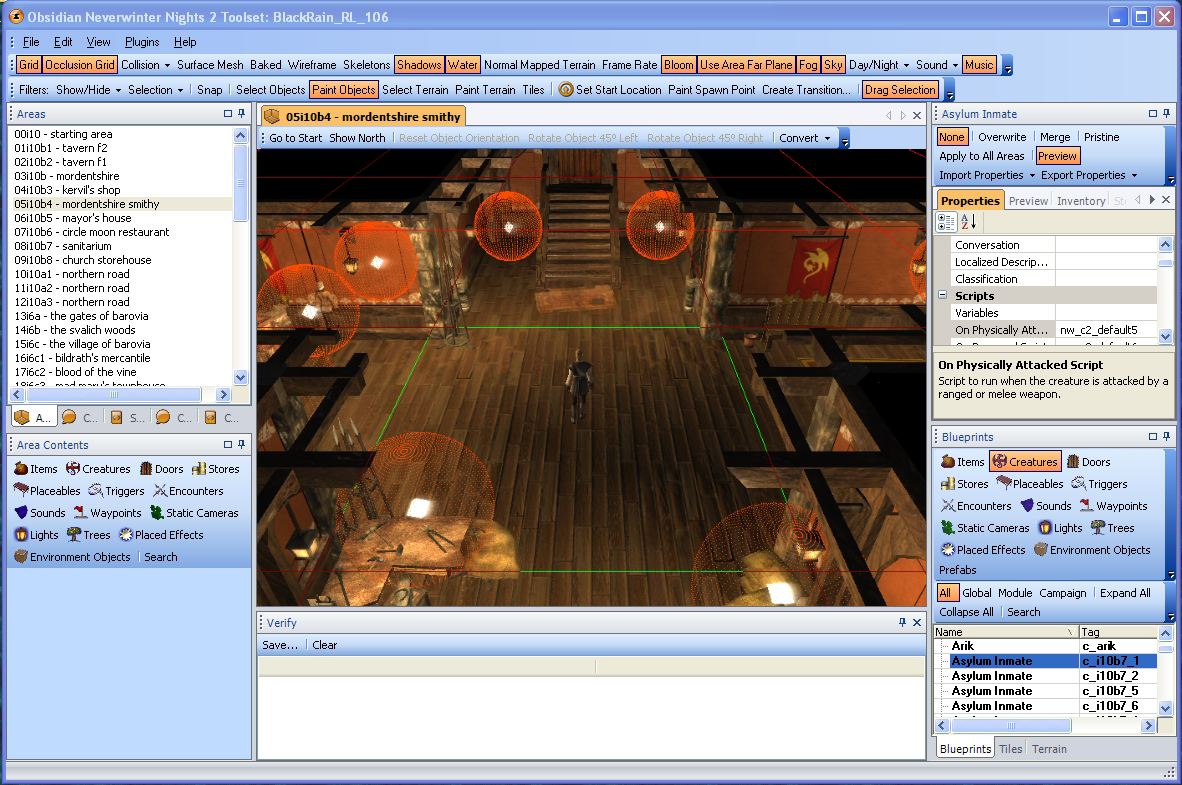
\includegraphics[width=0.527\textwidth]{media/NeverwinterNights2-editor}
	\caption{Spiel\protect\footnotemark[2]- und Editor\protect\footnotemark[3]-Ansicht des PC-Rollenspiels Neverwinter Nights~2.}
\end{figure}


Digitale Rollenspiele basieren häufig auf einem ähnlichen Regelwerk wie Pen-\&-Paper-Spiele. Die exakten Formeln werden in ein festes Regelwerk überführt, welches der Computer zur Evaluierung aller Werte und Möglichkeiten nutzen kann. Anders als bei PnP-Spielen wir den digitalen Spielen jedoch ein starker Fokus auf die visuelle Repräsentation gelegt \cite{Tychsen2006}. Diese visuelle Repräsentation ersetzt die imaginäre Spielwelt von PnP-Rollenspielen. Dadurch ist keine kontinuierliche Kommunikation und Synchronisation von Ereignissen und Umgebungen zwischen Spielleiter und Spielern mehr nötig \cite{Drachen2008}. Gleichzeitig geht ein Großteil der Kontrolle über den Spielverlauf vom Spieler an den Computer über. Der Spieler muss, anders als bei PnP-Spielen, nicht zwingend Verständnis über die Regeln des Spieles haben. Alle Entscheidungen werden im Hintergrund durch den Computer getroffen und in der visuellen Repräsentation reflektiert. Dieses strikte Vorgehen verhindert das variieren von Regeln. Während ein PnP-Spielleiter kreative Entscheidungen auf Basis der bekannten Regeln treffen kann, ist der Computer an exakt den vordefinierten Regelsatz gebunden. \cite{Drachen2008}

\footnotetext[2]{http://www.mobygames.com/game/windows/neverwinter-nights-2-mask-of-the-betrayer/screenshots/gameShotId,276723/, 20.03.2014}
\addtocounter{footnote}{1}
\footnotetext[3]{http://www.cs.cornell.edu/bigreddata/games/SGL.php, 20.03.2014}
\addtocounter{footnote}{1}

Als Beispiel sei das Rollenspiel \emph{Neverwinter Nights 2}\footnote{http://www.obsidian.net/games\#nwn2} von \emph{OBSIDIAN Entertainment} genannt, welches auf dem D\&D-Regelwerk der 3. Edition basiert. Mit einem mitgelieferten Editor ist es möglich ein eigenes Abenteuer zu erstellen und mit anderen Spielern über das Netzwerk zu spielen. Sogar rudimentäre Spielleiter-Tools sind vorhanden.~\cite{Tychsen2006a}



\section{Bestehende Ansätze}
\label{sec:BekannteAnsaetze}
%Paper und Programme die unserem Thema ähneln, jeweils mit Abgrenzung warum sie die Frage nicht zufriedenstellend (oder wenigstens schlechter als wir) beantworten können
%\begin{itemize}
%	\item RPG Maker
%	\item NWN
%	\item GM-AI
%	\item Tools die ähnliches leisten
%\end{itemize}

Das in \ref{sec:DigitaleRollenspiele} genannte \emph{Neverwinter Nights 2} wird mit einem Editor und einem Spielleiter-Tool ausgeliefert, welche das Erstellen und leiten eigener Abenteuer erlauben. Hierbei werden dem Spielleiter erweiterte Möglichkeiten in der Spielwelt zugesprochen, allerdings ist der Spielleiter dabei stets an die im Spiel implementierten Regeln gebunden und Spieler können nur genau die Aktionen ausführen, die von den Entwicklern implementiert wurden.~\cite{Tychsen2006a}\newline
Auch Tools die spezifisch zum Erstellen kleiner Rollenspiele entwickelt wurden wie der \emph{RPG Maker}\footnote{http://www.rpgmakerweb.com/} erreichen nicht die Handlungsfreiheit von PnP-Rollenspielen. Der RPG Maker erlaubt es dem Entwickler~/~Spielleiter neue Objekte zu erstellen und mit eigener Logik zu versehen. Nach der Distribution des RPGs ist der Spieler jedoch wiederum an das erdachte Regelsystem gebunden eine wirkliche Interaktion des Spielers und der Regelwelt des RPGs ist nicht möglich.\\
Die meisten aktuell vorhandenen Tools leiden unter dem Problem, dass die in \cite{Arinbjarnar} beschriebene dynamische Entwicklung der Geschichte nicht während des Spiels stattfinden kann. Eigene Regelsysteme und Questslinien müssen zumeist vor dem Abenteuer ausgearbeitet und finalisiert werden und während des Abenteuers hat die Spielergruppe nur marginalen Einfluss auf die Auslegung verschiedener Mechaniken.\newline
In der Forschung finden sich auch Ansätze um die Funktion eines Spielleiters durch ein Computersystem wahrnehmen zu lassen. \cite{Aylett2007} vergleicht die Arbeitsweise eines Spielleiters mit Problemen aus der Robotik. Aus vordefinierten Mustern müssen unter Berücksichtigung sich wechselnder Umwelteinflüsse die eigentlichen Handlungen konstruiert werden. Die Eckpunkte stellen im PnP-Kontext die vorher geplanten Geschichts-Eckpunkte dar, die Spielerentscheidungen während der Runde sind die äußeren, nicht planbaren Einflüsse.\newline
Diese \emph{digitalen Spielleiter} erzeugen Geschichten, Quests und Aktionen aus verschiedenen abstakten Regeln und sind damit in der Lage auf Entscheidungen der Spieler zu reagieren. \cite{Arinbjarnarb} gibt eine umfassende Übersicht über verschiedene Systeme dieser Art. Als Beispiel sei hier \emph{Directed Emergent Drama} (kurz \emph{DED}) \cite{Arinbjarnara} genannt, eine Spielform, in der einzelne Akteure von einem zentralen Programm angeleitet werden. DEDs nutzen so genannte Schemata um Charakteren verschiedene Rollen zuzuordnen. Je nach Zustand des Dramas vergibt der Regisseur verschiedene Schemata an die Akteure um die Geschichte voranzutreiben \cite{Arinbjarnarb}. Die Handlungen der Akteure und Spieler werden im Rahmen der zugeordneten Schemata analysiert und bei zu großen Abweichungen des aktuellen Schemas wird dieses von dem Direktor durch ein passenderes ersetzt \cite{Arinbjarnar}.\newline
Während dieser Ansatz eine dynamischere Reaktion auf Aktionen der Spieler ermöglicht ist die künstliche Intelligenz immer noch auf ihren Regelsatz beschränkt. Die Kreativität eines menschlichen Spielleiters, welche es erlaubt die Spielwelt während des Spiels konstant anzupassen, würde von dem Computer eine andauernde Evaluierung der Spieler-Aktionen und Umgestaltung der Spielwelt erfordern.\newline
Der in diesem Paper konzipierte Prototyp behandelt diese Probleme indem er dem Spielleiter die Möglichkeit gibt alle Objekte und ihre Eigenschaften zur Spielzeit frei zu manipulieren. Dies erlaubt es Spielern eigene, kreative Ideen in das Spiel einzubringen und dem Spielleiter diese Vorschläge bei Bedarf in das Spielsystem einzupassen. So erwächst bei jeder Spielrunde eine dynamische Spielwelt, welche den Anforderungen der Gruppe und des Abenteuers genügt.
